\documentclass{article}
\usepackage[utf8]{inputenc}
\usepackage{geometry}
\usepackage{graphicx}
\usepackage{pgfplots}
\usepackage{amsmath}
\usepackage{amssymb}
\usepackage{amsfonts}
\usepackage{mdframed}
\usepackage{amsthm}
\usepackage{tikz}
\usepackage{multicol}
\usepackage{cancel}

\geometry{a4paper, left=2cm, right=2cm, top=1cm, bottom=2cm}

\pgfplotsset{compat=1.18}
\begin{document}

\begin{minipage}{0.7\textwidth}
    \small \textbf{Fenómenos Colectivos}  \\
    \small {Facultad de Ciencias, Universidad Nacional Autónoma de México} \\
    \small {Profesora: Dra. Catalina Elizabeth Stern Forgach} \\
    \small {Ayudante: M. Tyra Delgadillo Mendoza} \\
    \small {Fecha de entrega: Lunes 12 de febrero del 2024} \\
    \small {Nombre completo: Andrés López González} \\
    \small {Recopilación: 1-7 Febrero}
\end{minipage}
\hfill
\begin{minipage}{0.12\textwidth}
    
\includegraphics[width=\linewidth]{logo_universidad}
\end{minipage}

\section*{Primera parte.}
I. Utilizando una escala apropiada.\\
$a)$ ¿Puedes, en una hoja de papel carta, dibujar un protón dentro de una cancha de football? \\
\textit{De acuerdo a los datos extraídos de la página oficial de la Liga Nacional de Fútbol Americano (NFL) su largo y ancho es de $120 \cdot 53.33$ yardas ($109.72 \cdot 48,76$ metros), mientras que de acuerdo a la Red de Revistas Científicas de América Latina y el Caribe, España y Portugal el diametro de un protón es de $1.2 \cdot 10^{-15}$ m. Suponiendo un plano bidimensional como lo es en este caso la hoja, utilizando la fórmula del área de un círculo obtenemos la siguiente área del protón proyectada en la hoja:}
\[ A_p = \frac{\pi d^2}{4} \approx (3.1416) \cdot \frac{(1.2 \cdot 10^{-15}m)^2}{4} \approx 1.13098 \cdot 10^{-30} m^2 \]
\textit{Ahora obtenemos el área de la cancha.}
\[ A_c \approx 109.72m \cdot 48.76m \approx 5349.95m^2\]
\textit{El siguiente paso posiblemente no sea bien visto, sin embargo los motivos refuerzan la necesidad de hacerlo pues comparar un área rectangular con una circular es absurdo. Supondremos que tanto la cancha como la proyección del protón sobre esta son cuadradas, para ello daremos las dimensiones de cuánto debería medir cada lado de estos dos cuadrados.}
\[ l_p = \sqrt{A_p} \approx \sqrt{1.13098 \cdot 10^{-30} m^2} \approx 1.06348\cdot 10^{-15}m\]
\[ l_c = \sqrt{A_c} \approx \sqrt{5349.95m^2} \approx 73.14335m\]
\textit{Obtenemos la razón entre áreas $\frac{A_{cancha}}{A_{protón}}$.}
\[ \frac{A_c}{A_p} \approx \frac{5349.95m^2}{1.13098 \cdot 10^{-30} m^2} \approx 4.73037\cdot 10^{33}\]
\textit{Finalmente obtenemos que suponiendo áreas de objetos cuadrados proyectadas en una hoja cuadrada (no carta pues los cálculos serían aún más infernales, no obstante, conservaría el mismo número de cuadrículas pero con figuras rectangulares en lugar de cuadradas) y teniendo cada cuadrícula a escala de cada lado correspondiente al lado del cuadrado del protón entonces necesitaríamos dividir la hoja en aproximadamente $4.73037\cdot 10^{33}$ partes de $1.06348\cdot 10^{-13}cm$ por lado cada cuadrícula.}\\\\
$b)$ ¿Hacer una línea de tiempo en la que aparezca tu edad, la edad de la Tierra y la edad del Universo? Si no puedes hacerlo, ¿Cuántas hojas necesitarías en cada caso?\\
\textit{Llevando el caso al absurdo como en el inciso a), intentaremos hacer esta línea del tiempo en una sola hoja. Para ello enlistamos los 3 datos requeridos en años (a):}\\
Edad propia $(E_p)$: 18 años\\
Edad de la tierra $(E_t)$: $4.543 \cdot 10^6$ años\\
Edad del universo $(E_u)$: $13.6 \cdot 10^9$ años\\
\textit{Consideramos mi edad como la mínima escala, deducimos las proporciones que existen entre mi edad y las demás}
\[ \frac{E_t}{E_p} \approx \frac{4.543 \cdot 10^6}{18} \approx 2.52388\:\cdot \:10^5 \]
\[ \frac{E_u}{E_p} \approx \frac{13.6 \cdot 10^9}{18} \approx  7.55555\:\cdot \:10^8\]
\textit{Tomamos el largo de la hoja tamaño carta (0.2794 m) como unidad representativa de la edad del universo, armamos una pequeña tabla de correspondencias}
\begin{align*}
    13.6 \cdot 10^9a &= \textit{1 hoja (27.94 cm)} \\
    4.543 \cdot 10^6a &= \frac{4.543 \cdot 10^6a}{13.6 \cdot 10^9a} \cdot 27.94cm \approx 9.33\:\cdot \:10^{-3} cm \\
    18a &= \frac{18a}{13.6 \cdot 10^9a} \cdot 27.94cm \approx 3.69794\:\cdot \:10^{-8}cm
\end{align*}
\textit{Teniendo esto y ordenando un poco los datos, ya hemos terminado de calcular cómo plasmar la línea del tiempo. Dividimos la hoja horizontalmente en $7.55555\:\cdot \:10^8$ partes de $3.69794\:\cdot \:10^{-8}cm$ cada una, para expresar mi edad uso una sola cuadrícula, para la edad de la tierra $2.52388\:\cdot \:10^5$ cuadrículas y la del universo $7.55555\:\cdot \:10^8$ lo cual es lo mismo que usar todo el largo.}

\section*{Segunda parte.}
II. ¿Cómo midió Eratóstenes el radio de la Tierra? \\
\textit{Eratóstenes fue un hombre de la época aproximadamente del siglo III a.C., midió el radio de la Tierra utilizando la geometría (relaciones trigonométicas que si bien no estaban nada maduras como se han consolidado en la actualidad, ya existían en el mundo antiguo) y la observación de la posición del Sol en dos ubicaciones diferentes de la superficie terrestre. Durante el solsticio de verano, midió la sombra de un obelisco en Siena (actual Asuán, Egipto), Eratóstenes notó que el Sol estaba directamente sobre la vertical en Alejandría (situada al norte). Utilizando la diferencia de ángulos resultante entre las sombras en ambas ciudades, pudo calcular la circunferencia de la Tierra. Conocía previamente la distancia entre ambas ciudades y, utilizando trigonometría, calculó que el ángulo entre los dos lugares era de aproximadamente 7 grados y 12 minutos. Esto para tal época ya era algo impresionante, sin embargo no se quedó ahí, los antiguos matemáticos griegos antes de Eratóstenes, como Arquímedes y Euclides, formaron las bases del entendimiento de la relación entre el diametro y la circunferencia, y habían realizado aproximaciones precisas de su valor (lo que denotamos actualmente como pi), este pequeño paréntesis es muy importante pues fue por esta relación que Eratóstenes pudo obtener el radio de la Tierra a partir de su circunferencia.} \\\\
\begin{figure}[h]
    \centering
    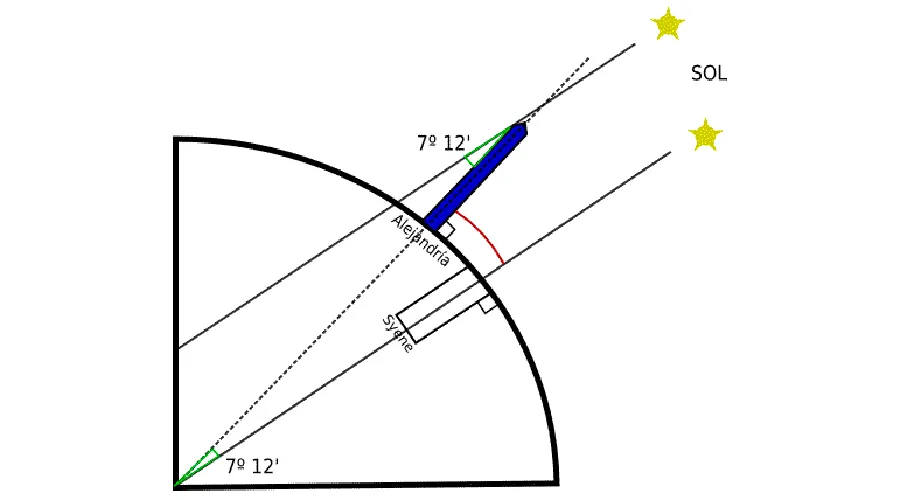
\includegraphics[width=0.5\linewidth]{Eratos.png}
    \caption{Geometría empleada por Eratóstenes}
    \label{fig:enter-label}
\end{figure}

III. ¿Cómo se mide la temperatura de una estrella? \\
\textit{En la actualidad existen dos métodos principales a través de los cuales se calcula la temperatura de una estrella.\\
(I) Análisis del espectro de emisión.\\
Los astrónomos descomponen la luz de una estrella utilizando espectrógrafos que separan la luz en diferentes longitudes de onda. Luego, detectan y amplifican estas señales utilizando detectores sensibles como CCDs (dispositivos de carga acoplada) y fotomultiplicadores, permitiendo el análisis detallado de las líneas espectrales. Las líneas espectrales son por nombrar de alguna manera la fingerprint (o  huella dactilar) de un compuesto químico, lo cual nos dice que entre cada compuesto o elemento químico este será distinto (en términos más técnicos nos dicen sus regiones de absorción y emisión de ondas electromagnéticas como la luz visible). Asímismo la intensidad de estas líneas espectrales nos dan información de la temperatura superficial de la estrella.}\\

\textit{(II) Brillo relativo en diferentes longitudes de onda.
Siendo este un poco menos impresionante porque el nombre nos dice todo, esta técnica se beneficia del brillo relativo en diferentes longitudes de onda como el infrarrojo, ultravioleta y la luz visible. Proporciona pistas sobre la temperatura de la superficie estelar mediante leyes como la ley de Wien y la ley de Stefan-Boltzmann.} \\
\begin{figure}[h]
  \centering
  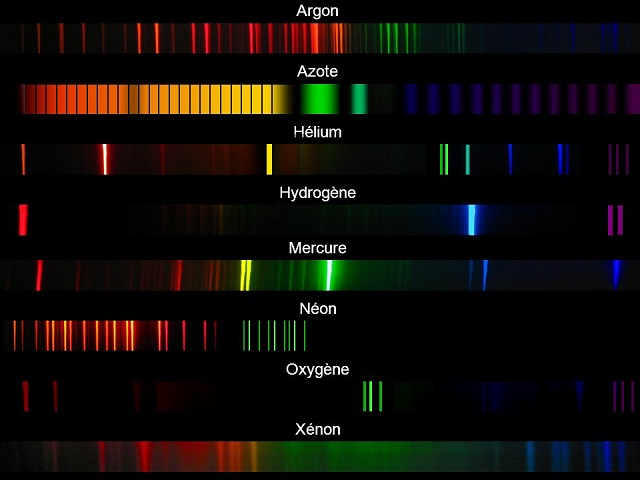
\includegraphics[width=8cm, height=6cm]{espectral.jpg}
  \caption{Espectros de emisión}
  \label{fig:espectral}
\end{figure}
\\
IV. ¿Cuál es la temperatura más baja que se ha podido medir? \\\\
\textit{En la Universidad de Stanford, Mark Kasevich y sus colegas utilizaron "lentes de onda-materia" (matter-wave lensing) para enfriar una nube de alrededor de 100,000 átomos de rubidio a menos de 50 pK (picokelvin = $kelvin \cdot 10^{-12}$). Siendo esto solo $5 \cdot 10^{-11}$ grados Kelvin por encima del cero absoluto. La temperatura de una nube de átomos se calcula con la velocidad promedio de los átomos a medida que se desplazan. El equipo de Kasevich utilizó una serie de lentes para reducir este movimiento promedio a menos de 70 µm/s, lo que corresponde a 50 pK. Esto rompe el récord anterior de 1 nK para las lentes de ondas de materia y representa el récord de la temperatura cinética más baja (record-low kinetic temperatures) según la reconocida Physical Review Letters, donde se describe más a profundidad la investigación; respecto a otros intentos de conseguir esta hazaña en 2011, Wolfgang Ketterle y sus colegas de la universidad Massachusetts Institute of Technology (MIT) lograron enfriar una red óptica de átomos de rubidio a aproximadamente 350 pK utilizando una técnica magnética. Mientras tanto, Pertti Hakonen y sus colegas de la Universidad Aalto en Finlandia lograron enfriar espines nucleares en una muestra sólida a unos fríos 100 pK en 2010, pero se podría argumentar que es sólo un grado de libertad y no es lo mismo que enfriar un gas. \\
Estas son las temperaturas más bajas que se han podido medir, no obstante, en lo personal es imposible pasar por alto la misión de Cold Atom Laboratory. Este laboratorio, lanzado a la Estación Espacial Internacional en marzo de 2018, usa láseres para enfriar átomos a menos de un grado para alcanzar el cero absoluto, cuando las nubes de átomos alcanzan estas temperaturas ultrafrías pueden formar un quinto estado de la materia llamado Condensado de Bose-Einstein (BEC). A diferencia de gases, líquidos, sólidos y plasmas, los CBE permiten la observación macroscópica de propiedades cuánticas, nunca nadie había producido antes estos CBE en órbita terrestre. Esta misión es operada remotamente desde el laboratorio "NASA's Jet Propulsion Laboratory", el objetivo de Cold Atom Lab es abrir nuevas vías de investigación sobre la naturaleza cuántica de los átomos en microgravedad, con potenciales aplicaciones en tecnologías cotidianas, aunque es bien sabido que estas temperaturas también favorecen a la creación de un superconductor pues a estas temperaturas los electrones forman pares de Cooper y al existir una resistencia casi nula pueden viajar libremente sin dispersión de la energía, mientras que por otro lado favorecen a los superfluidos como el Helio-4 que se comporta a estas temperaturas colectivamente como una sola entidad cuántica lo que le permite el flujo sin casi resistencia a través del material.}
\begin{figure}[h]
    \centering
    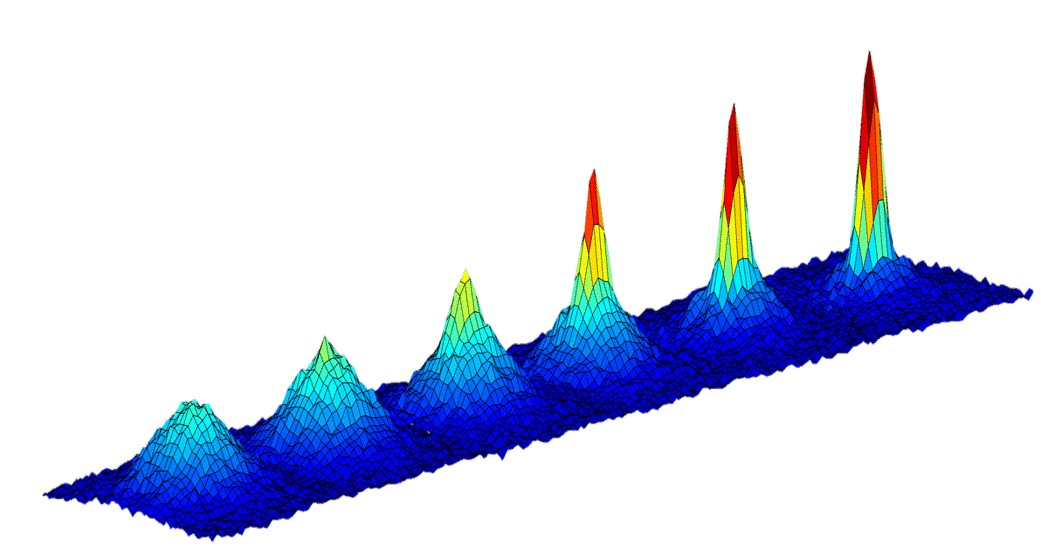
\includegraphics[width=0.45\linewidth]{CAL.png}
    \caption{This series of graphs show the changing density of a cloud of atoms as it is cooled to lower and lower temperatures (going from left to right) approaching absolute zero. The emergence of a sharp peak in the later graphs confirms the formation of a Bose-Einstein condensate [NASA]}
    \label{fig:enter-label}
\end{figure}
\newpage
\section*{Tercera parte.}
Si tu cabeza tiene un área de 100 $cm^2$, ¿cuál es la fuerza que ejerce la atmósfera sobre ella cuando estás a nivel del mar? Considérese $1atm = 101,325 Pa$ \\
\textit{Por la fórmula de la presión obtenemos.}
\begin{align*}
    P &= \frac{F}{A} \\
    F &= PA \\
    &= (1 atm\left[\frac{101,325Pa}{1 atm}\right])(100cm^2\left[\frac{1m^2}{10,000cm^2}\right]) \\
    &= (101,325\frac{N}{m^2})(0.01m^2) \\
    &= 1013.25 N
\end{align*}
¿Qué es el módulo de Young? \\
\textit{El módulo de Young es una propiedad de los materiales que describe su rigidez o capacidad para deformarse elásticamente cuando se le ejerce una fuerza. Representa la relación entre la tensión y la deformación (cambio en longitud respecto a la longitud original) en un material elástico. En otras palabras, cuanto mayor sea el módulo de Young, más rígido (o dificil de deformar) será el material. Se representa comúnmente por la letra \textbf{E} o \textbf{Y} y utiliza unidades de medida de presión, generalmente Pascales (Pa).} \\\\

Resuelve el problema 19 del capítulo 15 de la versión del Resnick que les compartí. \\
A U-tube of uniform cross-sectional area and open to the atmosphere is partially filled with mercury. Water is then poured into both arms. If the equilibrium configuration of the tube is as shown in Figure P15.19, with $h_2 = 1cm$, determine the value of $h_1$. \\
\textit{Consideremos un sistema hidrostático de presiones iguales.} \\
\begin{figure}[h]
    \centering
    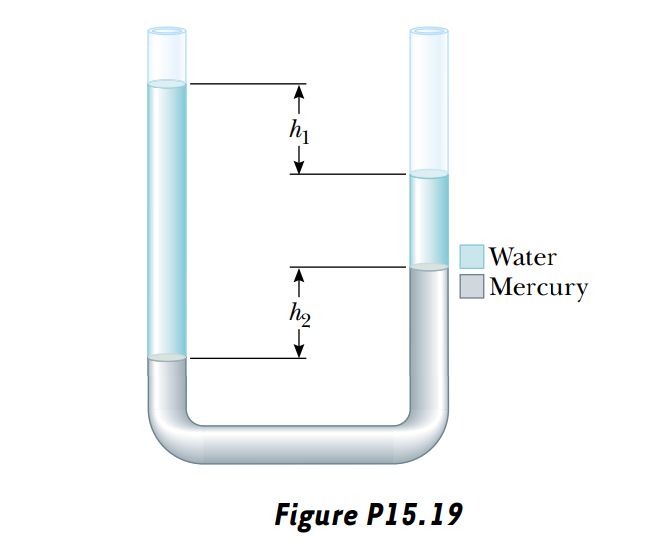
\includegraphics[width=0.45\linewidth]{ej1.png}
    \label{fig:enter-label}
\end{figure} \\
\begin{align*}
    P_1 &= P_2 \\
    P_0 + \rho_{a}g(h_1 + h_2 + h) &= P_0 + \rho_{a}gh + \rho_{hg}gh_2 \\
    \rho_{a}g(h_1 + h_2 + h) &= \rho_{a}gh + \rho_{hg}gh_2 \\
    h_1 + h_2 + h &= \frac{\rho_{a}gh + \rho_{hg}gh_2}{\rho_{a}g} \\
    h_1 + h_2 + h &= h + \frac{\rho_{hg}gh_2}{\rho_ag} \\
    h_1 + h_2 &= \frac{\rho_{hg}h_2}{\rho_a} \\
    h_1 &= \frac{\rho_{hg}h_2}{\rho_a} - h_2 \\
    h_1 &= \frac{[13.59\frac{g}{cm^2}]1.0cm}{1.0\frac{g}{cm^3}} - 1.0cm = 12.59cm
\end{align*}
\newpage
\textbf{PROBLEMA EXTRA DEJADO EN CLASE.} \\
Calcular el calor específico del siguiente material: Un recipiente de 3.6kg de este material contiene 14kg de agua, en esa agua se introduce un bloque de 1.8kg del mismo material a $180^{\circ}C$. Considera que la temperatura inicial del agua y del recipiente es de $16^{\circ}C$, la temperatura final es $18^{\circ}C$. \\\\
\textit{Para este problema denotaremos con subíndice uno a todo lo relacionado al primer sistema, mientras que el subíndice dos será el referente al bloque, se supondrá que el calor específico es constante por lo que no usaremos notación de integral. Debido a que es un poco ambigüo el enunciado asumiremos que el primer sistema ya ha alcanzado el equilibrio térmico por lo que considerar sus propiedades (calor específico, masa) será descartado en este análisis y se tomará solo en cuenta al agua de este primer sistema, esta decisión ha sido parcialmente inducida porque es imposible obtener el calor específico del material desconocido si ni siquiera sabemos el calor específico del sistema uno que en este caso sería un "combinado". Dicho esto usaremos una de las ecuaciones más importantes de la termodinámica para el calor en la que expresamos que el calor ganado de un sistema es el desprendido del otro, por ello el Q negativo.}
\begin{align*}
    Q &= -Q \\
    m_1c_1\Delta T_1 &= -m_2c_2\Delta T_2 \\
    c_2 &= -m_1c_1\Delta T_1[m_2\Delta T_2]^{-1} \\
    &= -m_1c_1(T_{f1}-T_{i1})[m_2(T_{f2}-T_{i2})]^{-1} \\
    &= \frac{-(14kg)\left(1\frac{kcal}{^{\circ}Ckg}\right)(18-16)^{\circ}C}{(1.8kg)(18-180)^{\circ}C} \\
    &= 0.096021 \frac{kcal}{^{\circ}Ckg} \\
    &= 96.02194 \frac{cal}{^{\circ}Ckg}
    \end{align*}

\end{document}